\documentclass{article}
\usepackage{arxiv}
\usepackage{pythonhighlight}

\usepackage[utf8]{inputenc} % allow utf-8 input
\usepackage[T1]{fontenc}    % use 8-bit T1 fonts
\usepackage{hyperref}       % hyperlinks
\usepackage{url}            % simple URL typesetting
\usepackage{booktabs}       % professional-quality tables
\usepackage{amsfonts}       % blackboard math symbols
\usepackage{amsmath}
\usepackage{nicefrac}       % compact symbols for 1/2, etc.
\usepackage{microtype}      % microtypography
\usepackage{graphicx}
\graphicspath{ {./images/} }
\usepackage{natbib}
\usepackage{doi}
\usepackage{listings}		% to include some code snippets
\usepackage{xcolor}

\definecolor{codegreen}{rgb}{0,0.6,0}
\definecolor{codegray}{rgb}{0.5,0.5,0.5}
\definecolor{codepurple}{rgb}{0.58,0,0.82}
\definecolor{backcolour}{rgb}{0.95,0.95,0.92}

% Default fixed font does not support bold face
\DeclareFixedFont{\ttb}{T1}{txtt}{bx}{n}{12} % for bold
\DeclareFixedFont{\ttm}{T1}{txtt}{m}{n}{12}  % for normal

\lstdefinestyle{mystyle}{
    backgroundcolor=\color{backcolour},   
    commentstyle=\color{codegreen},
    keywordstyle=\color{magenta},
    numberstyle=\tiny\color{codegray},
    stringstyle=\color{codepurple},
    basicstyle=\ttfamily\footnotesize,
    breakatwhitespace=false,         
    breaklines=true,                 
    captionpos=b,                    
    keepspaces=true,                 
    numbers=left,                    
    numbersep=5pt,                  
    showspaces=false,                
    showstringspaces=false,
    showtabs=false,                  
    tabsize=2
}


\lstset{style=mystyle}


\title{An initiation on community-driven peak-analysis GUI tool for spectroscopic data analysis (DRAFT)}

%\date{September 9, 1985}	% Here you can change the date presented in the paper title
%\date{} 					% Or removing it

\author{ \href{https://orcid.org/0000-0001-7670-300X}{
\includegraphics[scale=0.06]{orcid.pdf}\hspace{1mm}Kyunghoon Han}\thanks{Corresponding author. The GitHub repository on this tutorial is: } \\
	Department of Physics and Materials Science,\\
	University of Luxembourg,\\
	Luxembourg L-1511\\
	\texttt{kyunghoon.h@gmail.com} \\
	%% examples of more authors
	\And
	\href{https://orcid.org/0000-0002-6959-4607}{
\includegraphics[scale=0.06]{orcid.pdf}\hspace{1mm}Joshua T. Berryman} \\
	Department of Physics and Materials Science,\\
	University of Luxembourg,\\
	Luxembourg L-1511\\
	\texttt{josh.berryman@uni.lu} \\
    \And
	\href{https://orcid.org/}{
\includegraphics[scale=0.06]{orcid.pdf}\hspace{1mm}Ariadni Boziki} \\
	Department of Physics and Materials Science,\\
	University of Luxembourg,\\
	Luxembourg L-1511\\
	\texttt{josh.berryman@uni.lu} \\
    \And
	\href{https://orcid.org/}{
\includegraphics[scale=0.06]{orcid.pdf}\hspace{1mm}Alexandre Tkatchenko} \\
	Department of Physics and Materials Science,\\
	University of Luxembourg,\\
	Luxembourg L-1511\\
	\texttt{josh.berryman@uni.lu} \\
}

% Uncomment to remove the date
%\date{}

% Uncomment to override  the `A preprint' in the header
%\renewcommand{\headeright}{Technical Report}
%\renewcommand{\undertitle}{Technical Report}
\renewcommand{\shorttitle}{Tutorial on peak identification}

%%% Add PDF metadata to help others organize their library
%%% Once the PDF is generated, you can check the metadata with
%%% $ pdfinfo template.pdf
\hypersetup{
pdftitle={tutorial_peaks},
pdfsubject={q-bio.NC, q-bio.QM},
pdfauthor={Kyunghoon ~Han, Ariadni ~Boziki, Joshua T. ~Berryman, Alexandre ~Tkchatchenko},
pdfkeywords={Random matrices, IR spectroscopy, Raman spectroscopy, Physical Chemistry},
}

\begin{document}
\maketitle

\begin{abstract}
	In the domains of chemical and biological systems, scientist often grapple with deciphering signals derived from theoretical or experimental findings.
    This intricate process might involve disassembling the signal into distinct distributions or reconstructing it to yield a more authentic representation.
    For researchers entrenched in applied fields, this seemingly straightforward task can pose a significant challenge, demanding proficiency in both signal processing and programming.
    This tutorial is designed to provide a systematic, step-by-step guidefor crafting a Graphic User Interface (GUI) capable of pinpointing signal peaks,
    untangling the input signal into distributions, and visually displaying the resulting data.
\end{abstract}


% keywords can be removed
%\keywords{Spectroscopy \and Graphic User Interface \and Peak Detection \and Peak Identification \and others}

%
%   Introduction and Motivation
%
\section*{Introduction and Motivation}
IDEA: As I was adviced that a ``tutorial'' would not be good enough as a publication, I want to 
INTRODUCE WHY WE NEED COMMUNITY-MANAGED PEAK DETECTION GUI TOOLS.
1) COMMERCIAL TOOLS ARE TOO EXPENSIVE
2) THE ALGORITHMS THEMSELVES ARE NOT VERY DIFFICULT
3) WE NEED A TOOL WHERE THE USERS CAN MODIFY ACCORDING TO THEIR NEEDS
%
%   Theoretical Recaps
%
\section{Theoretical Recaps}
\label{sec:1}
This section is composed of three subsections: peak-identification methods, detrending algorithms, decomposition of the signal to a sum of distributions.
For those aiming to bypass the theoretical aspects and dive directly into GUI development, please proceed to the Section \ref{sec:2}.

The main tutorial provided in the GitHub repository also contains a tutorial on the signal denoising and refinement methods.
These are important topics as well, however, authors would like to spend more time on GUI application stage as much as possible.

If the reader's interested: READ THE REFERENCES TO BE ADDED (wavelet transforms etc.).
%
%   Peak detection method
%
\subsection{Peak detection method}
A straightforward peak-detection algorithm entails a two-step procedure: 
identifying a local maximum within a specified window among the potential candidates where the negative of the second derivative of the signal reaches a local maximum.
However, it's important to note that a signal might be comprised of multiple sections that are not entirely disjoint.

Defining the window for this algorithm is crucial.
The window's definition typically involves determining its size and establishing the degree to which two neighboring windows can overlap. 
This methodology aims to encapsulate signal variations effectively while allowing for seamless transitions between sections.
The intuition behind this lies in ensuring that the window size is optimal for capturing peaks while accommodating potential variations within the signal's structure and content.
Defining a number of different windows for the entire signal with constant window-size will give an illusion that the window is propagating from one end of the signal to the other.
Hence, the method is called window-propagation method. 

A smaller window size generates more candidate peaks from the signal compared to a larger window size.
This is due to the increased likelihood of the amplitude corresponding to the median of the window reaching its maximum in a smaller window. 
Consequently, users are required to set a threshold based on the difference between the maximum and minimum amplitudes within the specified interval.
This threshold helps filter out peaks with insignificant height, improving the accuracy of the analysis.
The Figure \ref{fig:peak_detection} presents a sample outcome obtained using the aforementioned method, visually illustrating the imperative need for optimizing various window sizes and thresholds in the process.
\begin{figure}[hbt!]
    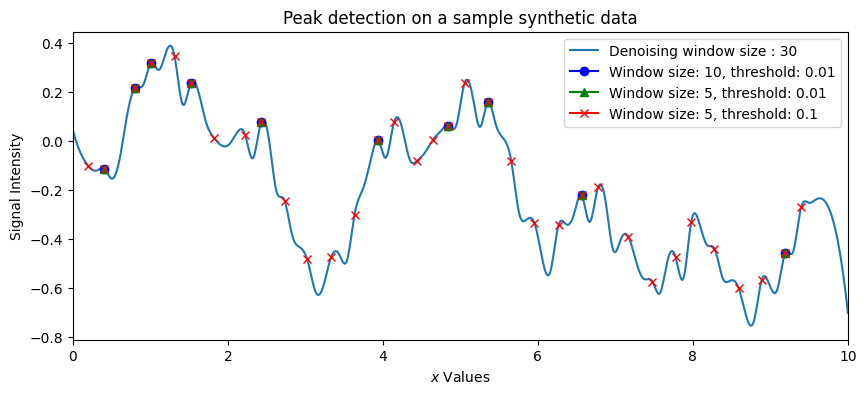
\includegraphics[width=\linewidth]{peak_detection.png}
    \caption{Visualization of a synthetic signal undergoing various peak-detection runs. A reduced window size and elevated threshold result in a higher count of potential peaks. Nonetheless, this trade-off increases the likelihood of including peaks generated by noise in the candidate list.}
    \label{fig:peak_detection}
\end{figure}


%
%   Signal detrending algorithms
%
\subsection{Signal detrending algorithms}
Signal detrending, also known as baseline correction, plays a pivotal role in comprehending spectral data's nature.
Accurate decomposition of spectral data relies on ensuring that the baseline aligns with the $x$-axis. 
However, one inherent challenge lies in the ambiguous definition of the so-called baseline.

In mathematical terms, a baseline can be defined as a function $B:\mathcal{D}(f) \rightarrow \mathcal{R}(f)$, where
\begin{equation*}
B = \min\left\{ f(x) : x \in U \subset \mathcal{D}(f), \text{ where $U$ is connected}\right\}
\end{equation*}
Here, $\mathcal{D}(f)$ and $\mathcal{R}(f)$ represent the domain and range of the function or distribution $f$.
It's important to note that $B$ isn't unique based on this definition.
What we ascertain from this definition is that $f(x) - B(x)$ yields a function that measures the deviation or alteration from the initial value of interest.

As the baselines are not unique, there are a number of different types of baseline correction algorithms: linear, Shirley backgrounds, penalized least squares (PLS), polynomial fittings, derivative methods, peak-clipping, etc.
In this section, the authors will introduce three simple algorithms: linear, adaptive iteratively reweighted PLS (airPLS) and asymmetrically reweighted PLS (arPLS).

The linear baseline algorithm represents the most straightforward approach.
It involves drawing a straight line connecting the initial coordinates to the signal's end-point.
This method is fast and less susceptible to distorting the signal's shape.

Yet, researchers might seek a nonlinear baseline or may aim to reshape the signal to remove noise from the profile. 
This is where PLS algorithms prove beneficial.
These algorithms are efficient, straightforward for debugging, and offer the flexibility required for accommodating nonlinear baselines and refining signal shapes during denoising processes.

The PLS algorithms establish the baseline as a vector, call it $\mathbf{z}$ as done in the work of Baek et. al (REFarPLS), achieved through minimizing the regularized least squares function, or the cost-function, defined below:

\begin{equation}
    \label{eq:pls}
    S(\mathbf{z}) = (\mathbf{s} - \mathbf{z})^T \mathbf{W}(\mathbf{s} - \mathbf{z}) + \lambda \mathbf{z}^T\mathbf{D}^T\mathbf{D}\mathbf{z}.
\end{equation}
Here, $\mathbf{D}$ represents the difference matrix
\begin{equation*}
    \mathbf{D} = \begin{bmatrix}
        1 & -2 & 1 & 0 & \cdots & 0 & 0 & 0 \\
        0 & 1 & -2 & 1 & \cdots & 0 & 0 & 0 \\
        \vdots & \vdots & \vdots & \vdots & \cdots & \vdots & \vdots & \vdots \\
        0 & 0 & 0 & 0 & \cdots & 1 & -2 & 1 
    \end{bmatrix},
\end{equation*}
$\mathbf{s}$ signifies the signal under analysis, while the matrix $\mathbf{W}$ and the scalar $\lambda$ serve as parameters to fine-tune.
The fitness to the data and the smoothness of the baseline are represented in the first and the second terms of the Equation \ref{eq:pls}, respectively REFarPLS.
The distinction between different least-squares methods are done by the choice of the parameters in the matrix $\mathbf{W}$.
\begin{equation*}
    w_i(n) = \begin{cases}
        0, &  s_i \geq z_i \\
        e^{n(s_i - z_i)/\| \mathbf{d} \|}, &  s_i < z_i\\
    \end{cases}
\end{equation*}
where $n$ is the iteration step, $s_i$ is the $i$-th component of the signal, $z_i$ is the $i$-th component of the baseline, and $\mathbf{d}$ is the negative elements of $\mathbf{s} - \mathbf{z}$.
Below is the implementation of the airPLS algorithm in Python 3, featuring the definition of $\mathbf{W}$ parameters.
The rationale behind the weight selections in this method is twofold: firstly, preserving whatever is already above the baseline, and secondly, iteratively updating weights exponentially to extend into the region beyond the baseline when $s_i$ falls below it.

The arPLS algorithm is expressed below, defining the parameters $\mathbf{W}$ as follows:
\begin{equation*}
    w_i(n) = \begin{cases}
        \left(1+ e^{2(d - (2 \sigma - \mu)/\sigma)}\right)^{-1}, &  s_i \geq z_i \\
        1, &  s_i < z_i\\
    \end{cases}
\end{equation*}
Here, $\sigma$ represents the standard deviation, and $\mu$ signifies the mean of the negative values of $\mathbf{s}-\mathbf{z}$.
In contrast to airPLS, this method aims to drive the logistics function (when $s_i \geq z_i$) towards convergence at 1.
This adjustment ensures that the majority of baseline values lie beneath the signal, resulting in a primarily positive detrended signal.
As a consequence, this method yields results closer to scientists' expectations from spectroscopic data.


The Figure \ref{fig:detrending} compares the abovementioned three baseline correction methods and illustrates the difference between the airPLS and arPLS results.
\begin{figure}[hbt!]
    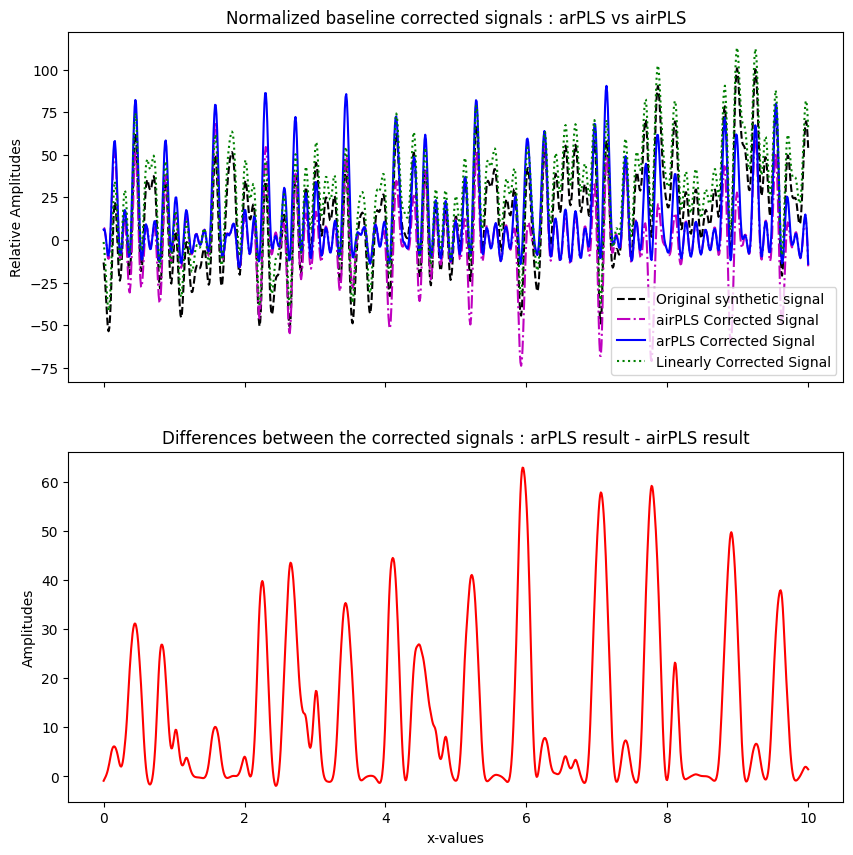
\includegraphics[width=\linewidth]{detrending_plots.png}
    \caption{Top: Comparison between the original, linearly detrended, airPLS-based detrended, and arPLS-based detrended signals. Bottom: Difference between the arPLS and airPLS results, showing the differences the two baseline correction methods can yield. Note that the positions of the peaks are not altered despite the changes in amplitudes. }
    \label{fig:detrending}
\end{figure}
%
%   Decomposition into multiple distributions
%
\subsection{Decomposition into multiple distributions}
The primary objective of the tasks detailed in the preceding two subsections is to generate a series of distributions that, when combined, form the corrected signal.
This corrected signal, obtained by subtracting the baseline, facilitates the recreation of the original input signal.
Many chemical or biological signals can be conceptualized as composite distributions of a similar type, often represented by Gaussians, Lorentzian/Cauchy, or Voigt distributions.
These individual distributions frequently correspond to specific signatures or components that researchers aim to investigate within the overall signal.

To start the discussion on how this can be done, first suppose we already have a denoised and detrended signal, $\hat{s}$, with peaks already identified.
Note first that the peaks are defined to be the local maxima with heights greater than certain threshold, where this threshold may vary according to the kind of signal one's interested in.
The problem our program needs to solve to obtain the decomposition is to find the parameters, $\mathbf{p}$, that can satisfy the following equality.
\begin{equation}
    \label{eq:decomposition}
    \hat{s}(\mathbf{x}) = \sum_{x_p\in \text{ peaks}} \mathcal{V}(\mathbf{x};\left\{x_p, \mathbf{p}\left(x_p\right)\right\})
\end{equation}
Where $\mathcal{V}$ can be one of Gaussian, Lorentzian or Voigt distributions.
Note the parameter's dependence on the peaks, $x_p$.
This is the case as the distributions corresponding to the different peaks have different shapes and sizes.

Similar to baseline correction, the parameters defining the distributions mentioned earlier are determined by optimizing a specific type of cost function.
The simplest function for optimization involves measuring the discrepancy between the targeted sum and the original signal sought. It can be represented as:
\begin{equation*}
    S(\mathbf{x}) = \left\|\hat{s}(\mathbf{x}) - \sum_{x_p\in \text{ peaks}} \mathcal{V}\left(\mathbf{x};\left\{x_p, \mathbf{p}\left(x_p\right)\right\}\right) \right\|^2
\end{equation*}
The objective is to minimize $S(\mathbf{x})$, ideally achieving a value of zero.
Although reaching zero is highly improbable, the aim is to get as close as possible, especially if the signal $\hat{s}$ maintains positive definiteness and continuity within a bounded set.
In spectroscopic applications, this set usually represents an interval where the signal is defined.
Determining the parameters involves identifying the minima of $S$ by computing the partial derivatives of $S$ concerning the parameters $\partial S / \partial \mathbf{p}$.
This famous optimization approach is commonly known as the least-squares optimization algorithm.

The least-squares algorithm presents a user-friendly approach for community engagement while ensuring efficiency.
Its simplicity has led to numerous enhancements documented in various journals, positioning it as an optimal optimization method for the community. (REFERENCES)

Despite its advantages, the community retains the flexibility to opt for alternative optimization algorithms.
One compelling reason for exploring other options is the challenging nature of parallelizing the least-squares algorithm.
While the parallelization of the method is not inherently complex, achieving accurate outputs from the parallelized process poses a significant challenge.
\begin{figure}[hbt!]
    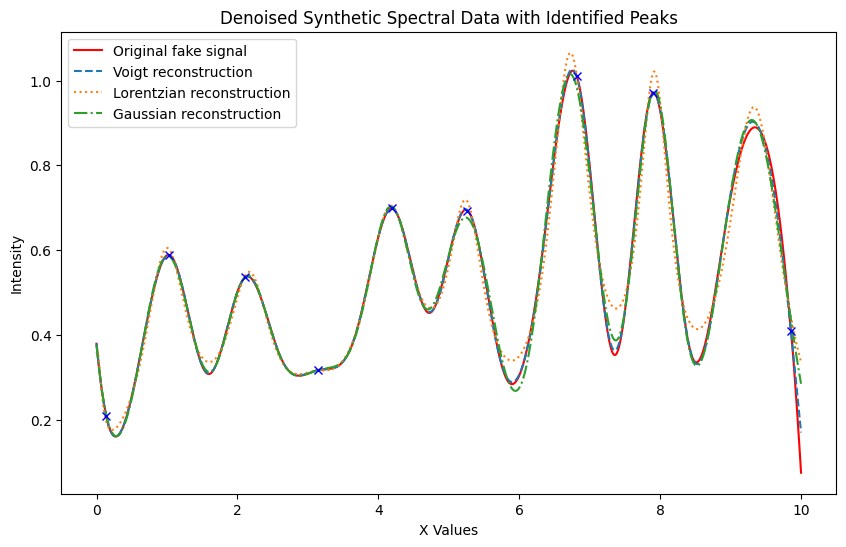
\includegraphics[width=\linewidth]{distribution_fitting.png}
    \caption{Demonstration of fitting spectral data through diverse distributions employs the least-squares method for the optimization of distribution parameters, contributing to the synthesis of the original signal.}
    \label{fig:detrending}
\end{figure}

%%%%%%%%%%%%%%%%%%%%%%%%%%%%%%%%%%%%%%%%%%%%%%%%%%%%%%%%%%%%%%
%%%%%%%%%%%%%%%%%%%%%%%%%%%%%%%%%%%%%%%%%%%%%%%%%%%%%%%%%%%%%%
%%%%%%%%%%%%%%%%%%%%%%%%%%%%%%%%%%%%%%%%%%%%%%%%%%%%%%%%%%%%%%
%%%%%%%%%%%%%%%%%%%%%%%%%%%%%%%%%%%%%%%%%%%%%%%%%%%%%%%%%%%%%%

%
%   The Application
%
\section{The Application}
\label{sec:2}

Though the tools outlined in Section \ref{sec:2} may initially appear unrelated, directing attention towards the goal of identifying peaks and distributions that collectively form the physically accurate signal reveals a coherent workflow.
By applying this approach to spectroscopic or other signal types, readers can discern the simplicity and effectiveness of the workflow.
The Figure \ref{fig:workflow} provides a visual representation of the strategic arrangement of these tools, showcasing the process by which one can systematically extract precise peak information from any given spectroscopic dataset.
The design is deliberately modular, enhancing its adaptability for future community-driven enhancements and streamlined debugging processes.
\begin{figure}[hbt!]
    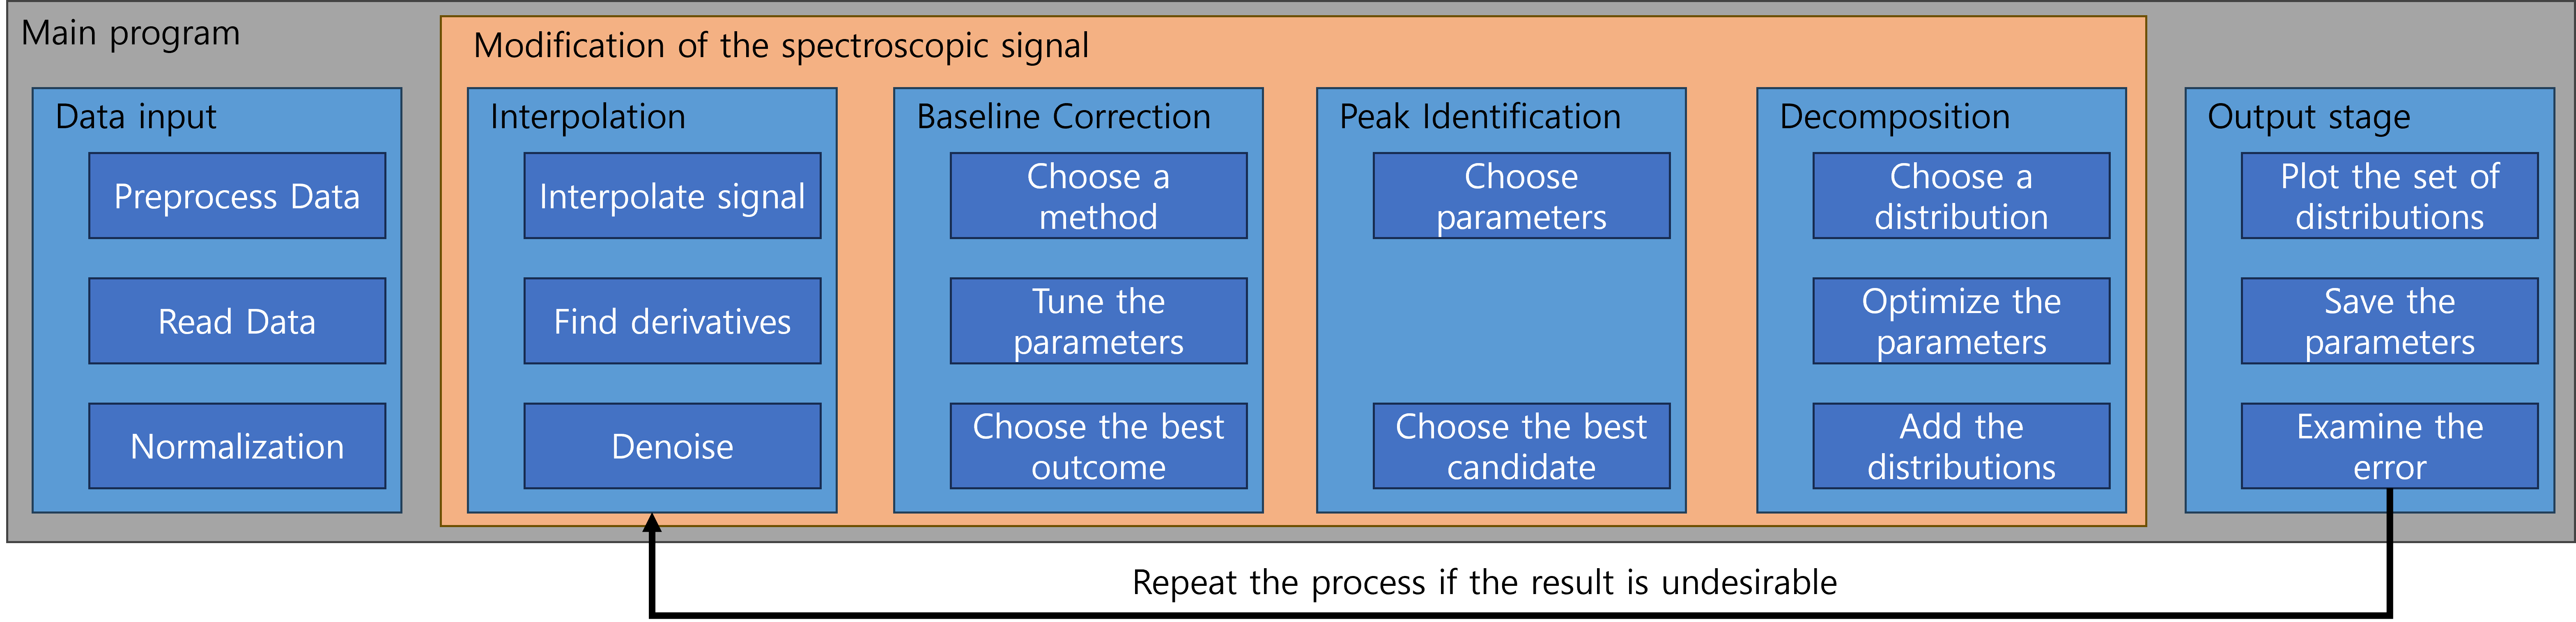
\includegraphics[width=\linewidth]{workflow.png}
    \caption{Illustrating a straightforward workflow for peak identification and distribution optimization, the four intermediate blocks can be executed independently of the main program, allowing users to treat each step as a distinct process. In the upcoming section, the GUI program introduces a wizard window that specifically addresses the highlighted orange components, providing users with transparent insights into the processes occurring beneath the GUI interface.}
    \label{fig:workflow}
\end{figure}
%
%   Main Section : basic UI for graphing
%
\subsection{Main section: basic UI for visualizing the input signal}
The program's core functionality centers on two pivotal tasks: 1) managing the input and output of signal data, and 2) presenting visualizations of pre-processed and modified results.
The primary aim of the main window is to execute these tasks efficiently while maintaining user intuitiveness.
Achieving this intuitiveness involves minimizing the number of buttons and interaction menus within the main interface.
By referring to Figure \ref{fig:main_window}, readers can readily observe that the UI is structured to guide users with limited selections, preventing any confusion or difficulty in navigating the program.
\begin{figure}[hbt!]
    \centering
    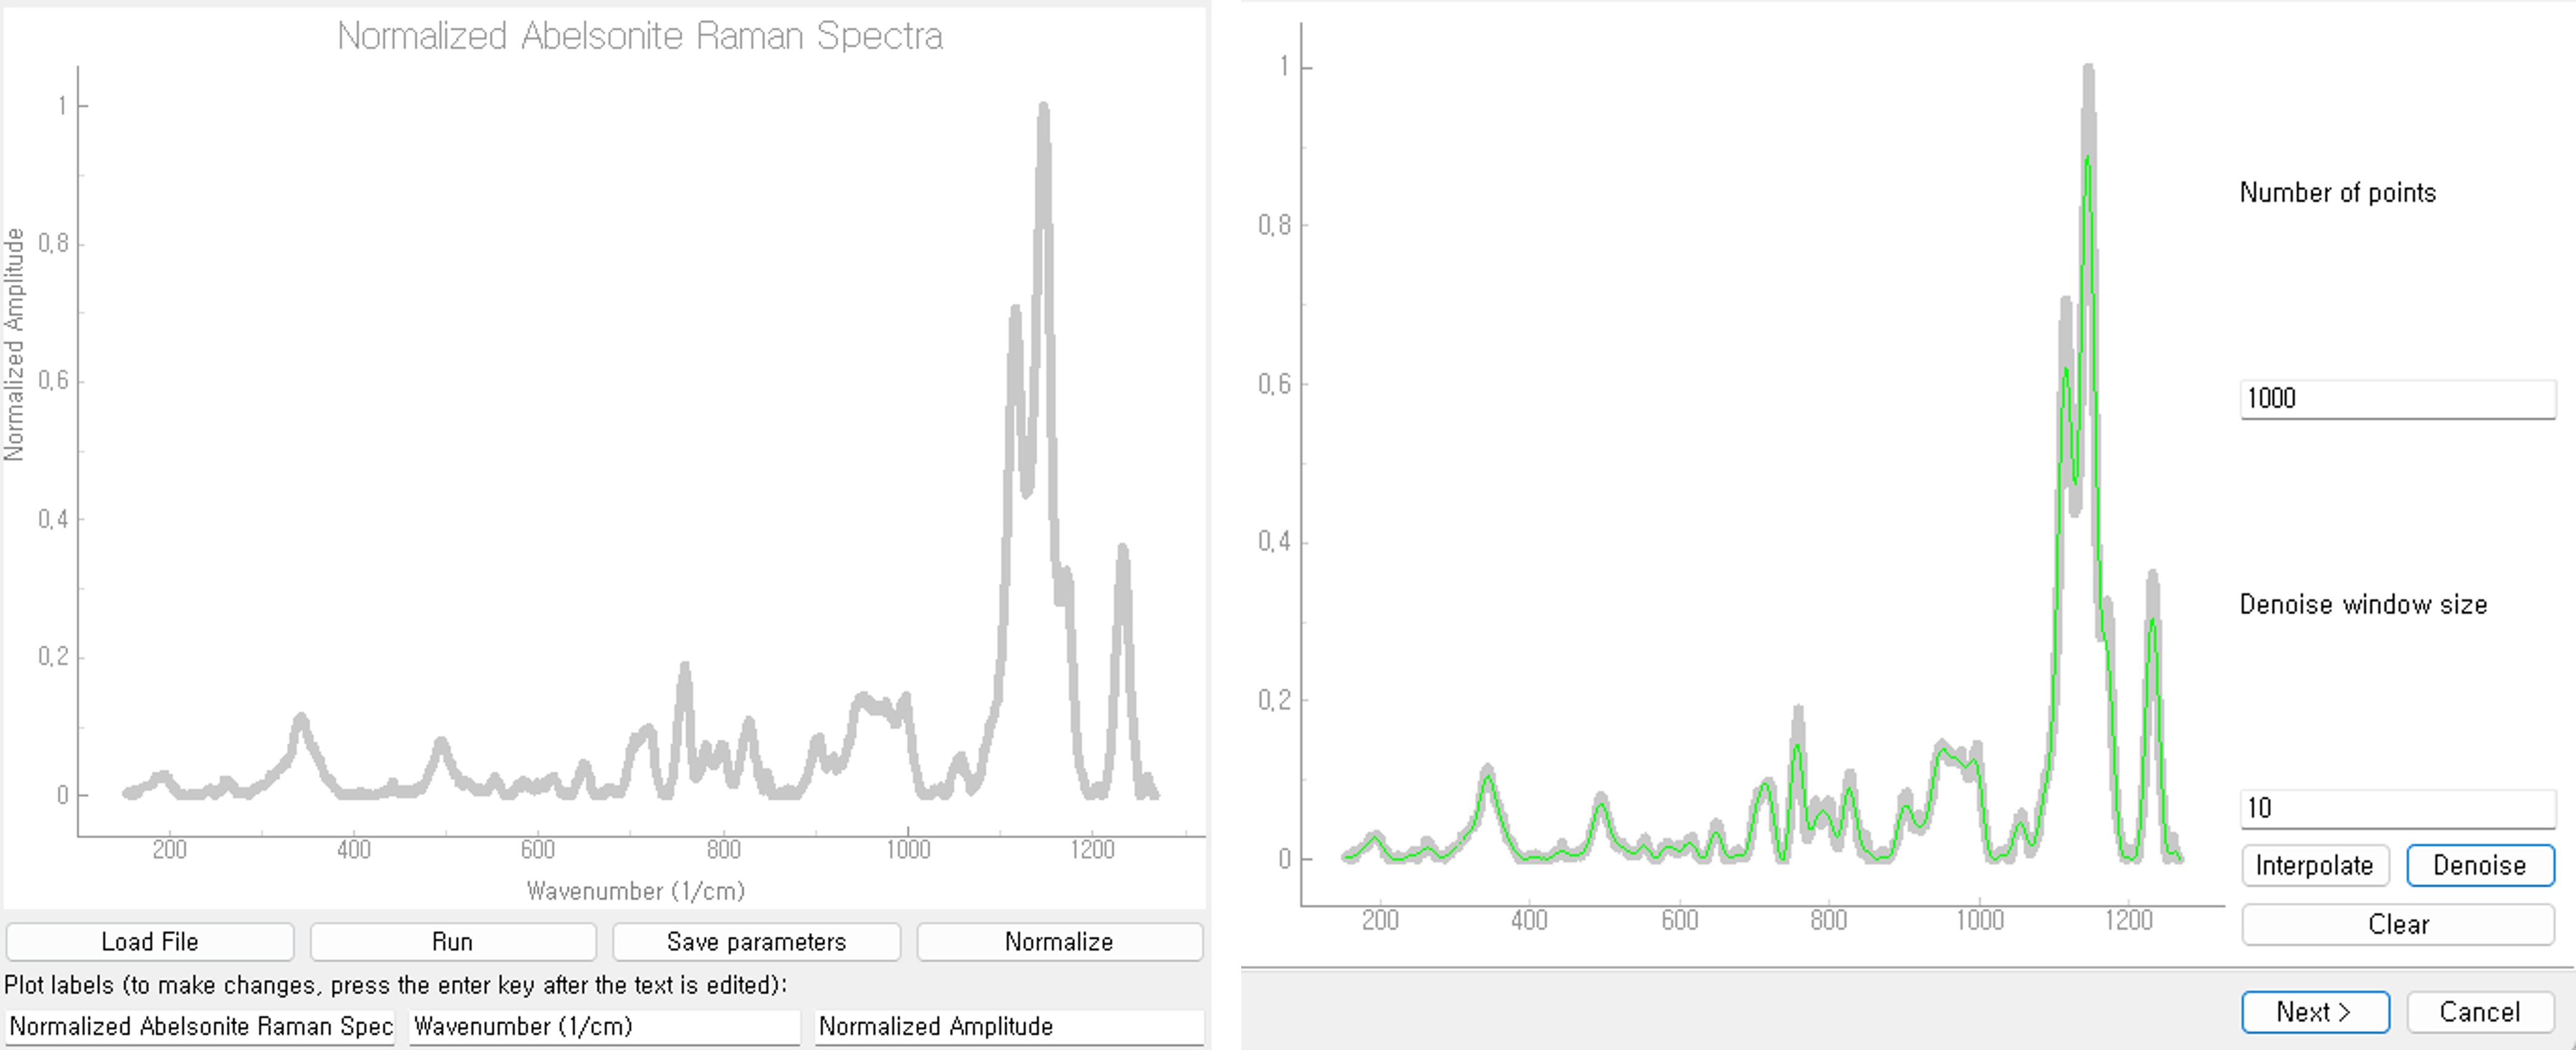
\includegraphics[width=\linewidth]{main_window.png}
    \caption{LEFT: The main window of the GUI, featuring a clean and straightforward interface with a minimal selection of buttons: load, run algorithm, save parameters, and normalize plot. Additionally, it provides an option to customize plot labels. Users can conveniently save data as a text file or export the plot as an image by utilizing the built-in functionality of \lstinline{PyQtGraph} library through a right-click on the plot. The showcased sample plot is sourced from the RRUFF database \cite{rruff}.
    RIGHT: Right: The wizard window the user is brought to upon pressing the \lstinline|Run| button. The green curve shows the result of denoising the input signal.}
    \label{fig:main_window}
\end{figure}

%
%   Wizards : main section where magic happens
%
\subsection{Wizards: the main analysis}
Upon pressing the \lstinline|Run| button, the users are brought to the interpolation and denoising section of the program.
This part is straightforward as the user is only expected to choose the parameters and see how their signal is being denoised.
Consult the Figure \ref{fig:main_window} for the illustrated explanation.

The \lstinline|Next| button then brings the users to a window with an option to select the baseline correction algorithm and to apply them.
There are only three selections to make on this section: type of baseline correction algorithm to apply, the lambda parameter for PLS methods and the ratio for the airPLS method.
The results obtained from this window is presented in the Figure \ref{fig:baseline_window}.
\begin{figure}
    \centering
    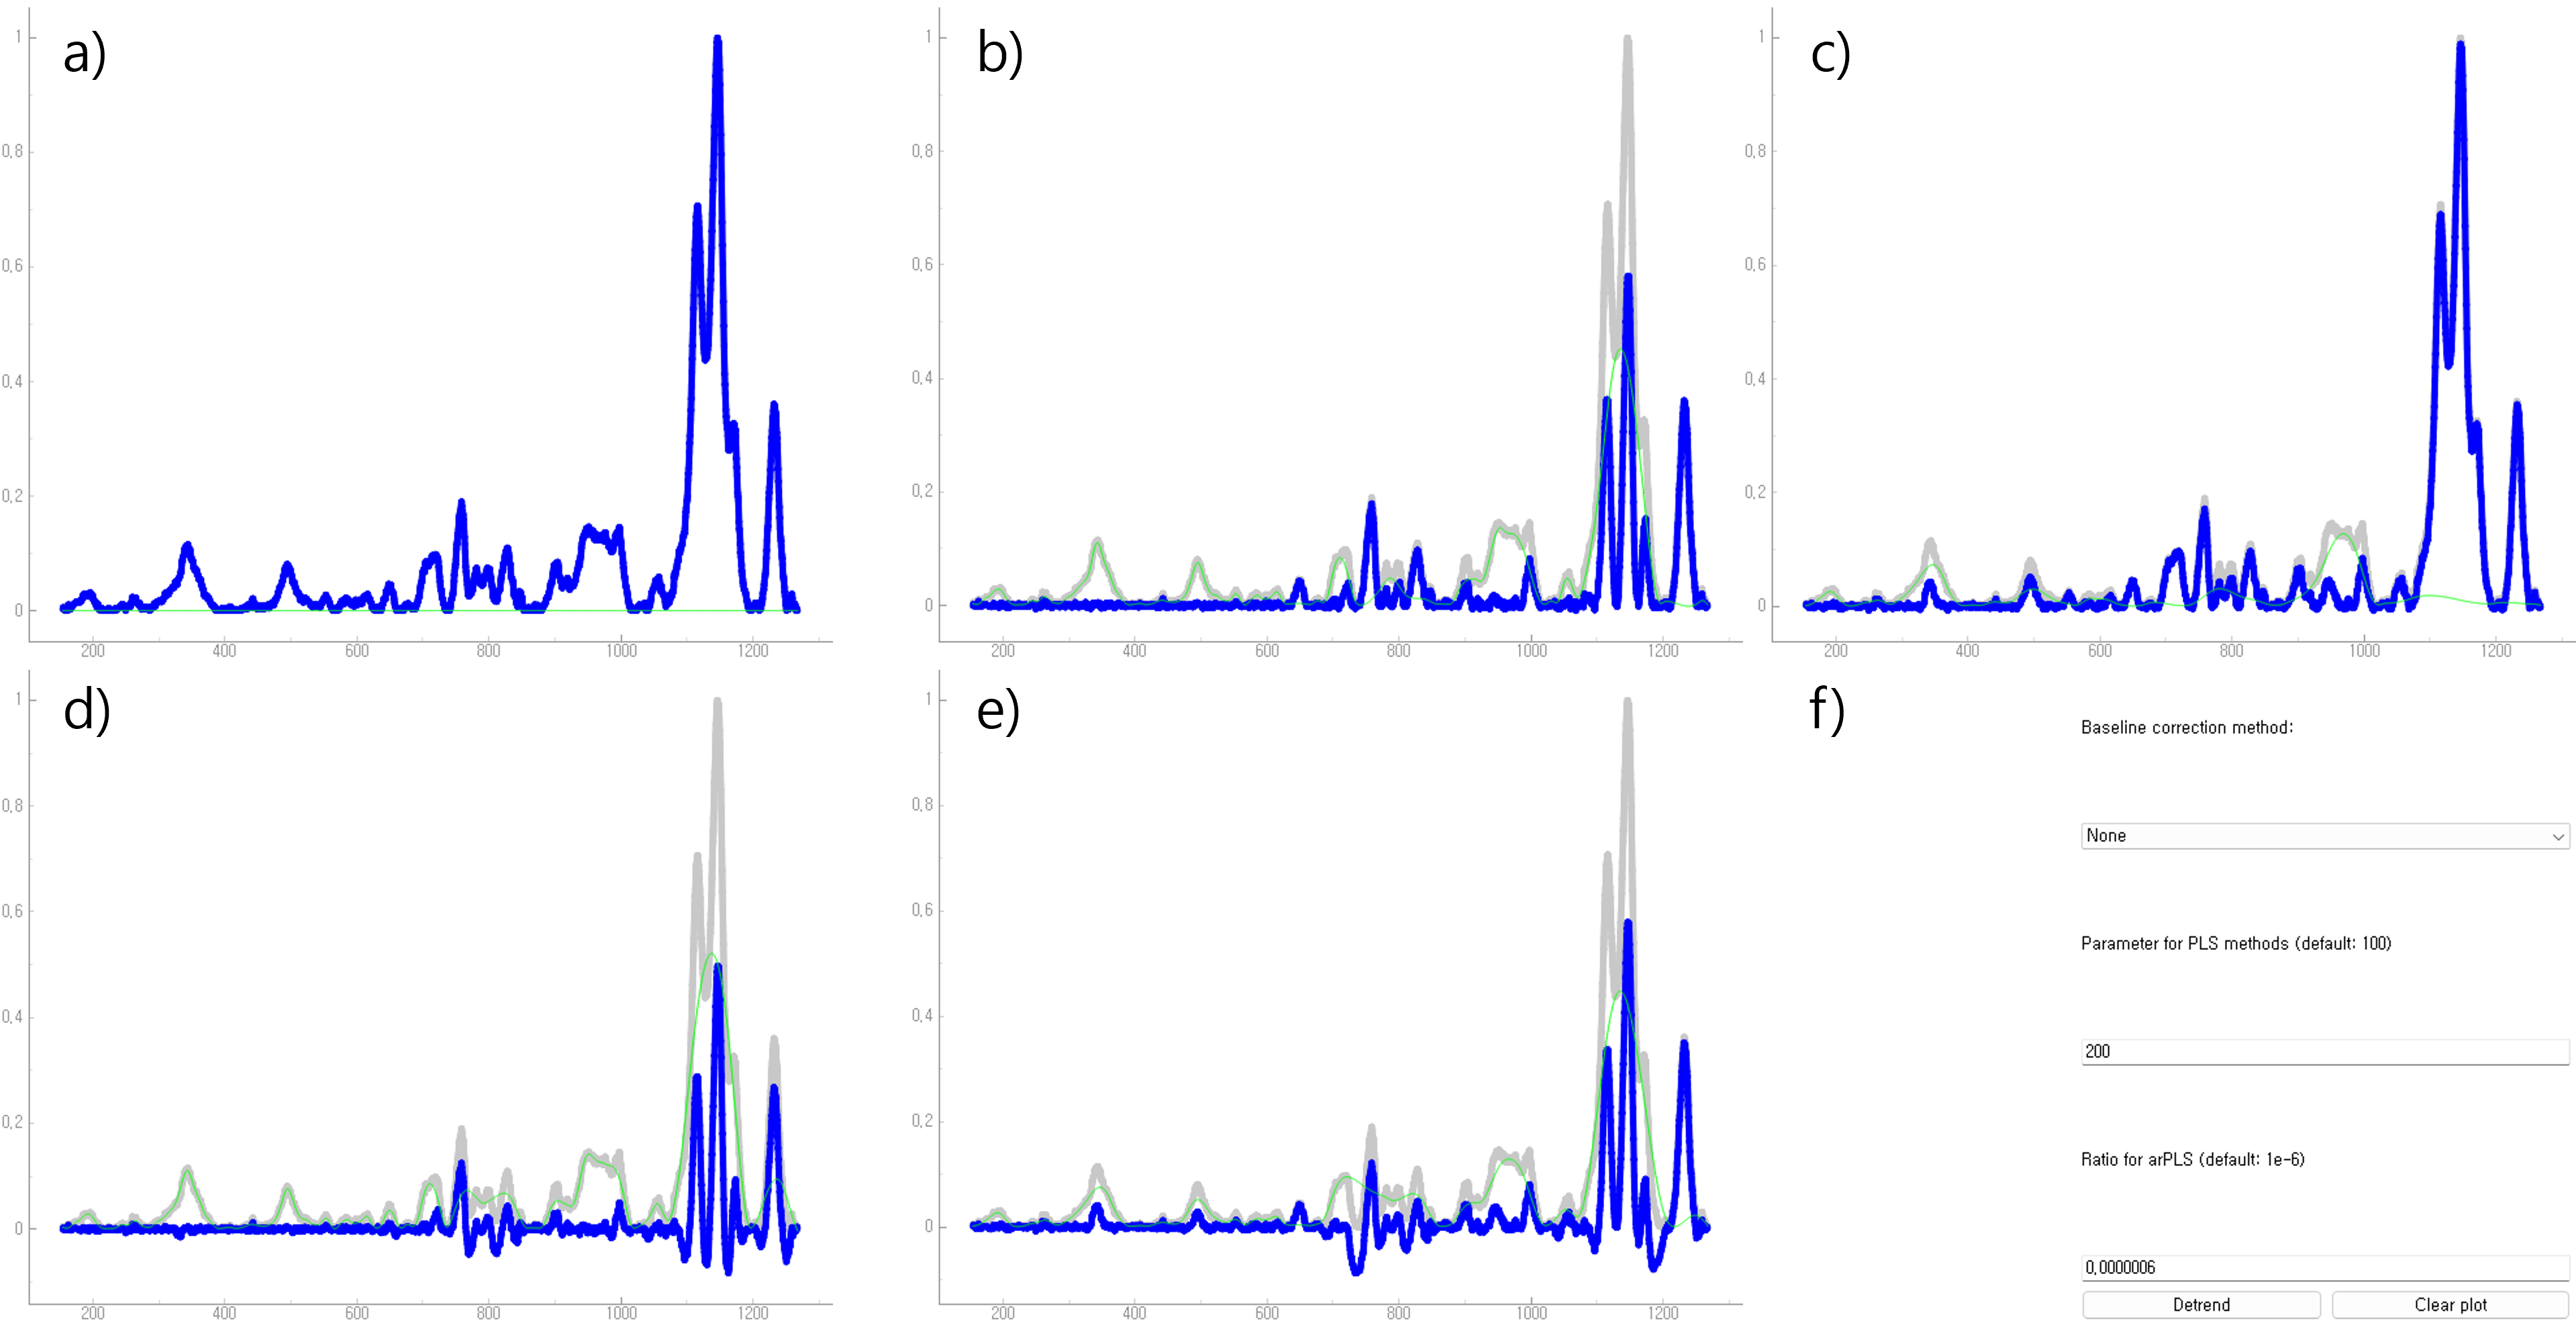
\includegraphics[width=\linewidth]{baseline_correction_window.png}
    \caption{a) Linear baseline correction result, b-c) arPLS baseline correction result with $\lambda=10^4$ and $\lambda=10^3$, respectively, d-e) airPLS baseline correction result with $\lambda=10^4$ and $\lambda=10^3$, respectively, and f) the menu the user has to toggle on the baseline-correction window.}
    \label{fig:baseline_window}
\end{figure}

The next two steps are straightforward. 
The Figure \ref{fig:last_two_windows} shows how these two last steps are processed.

\begin{figure}
    \centering
    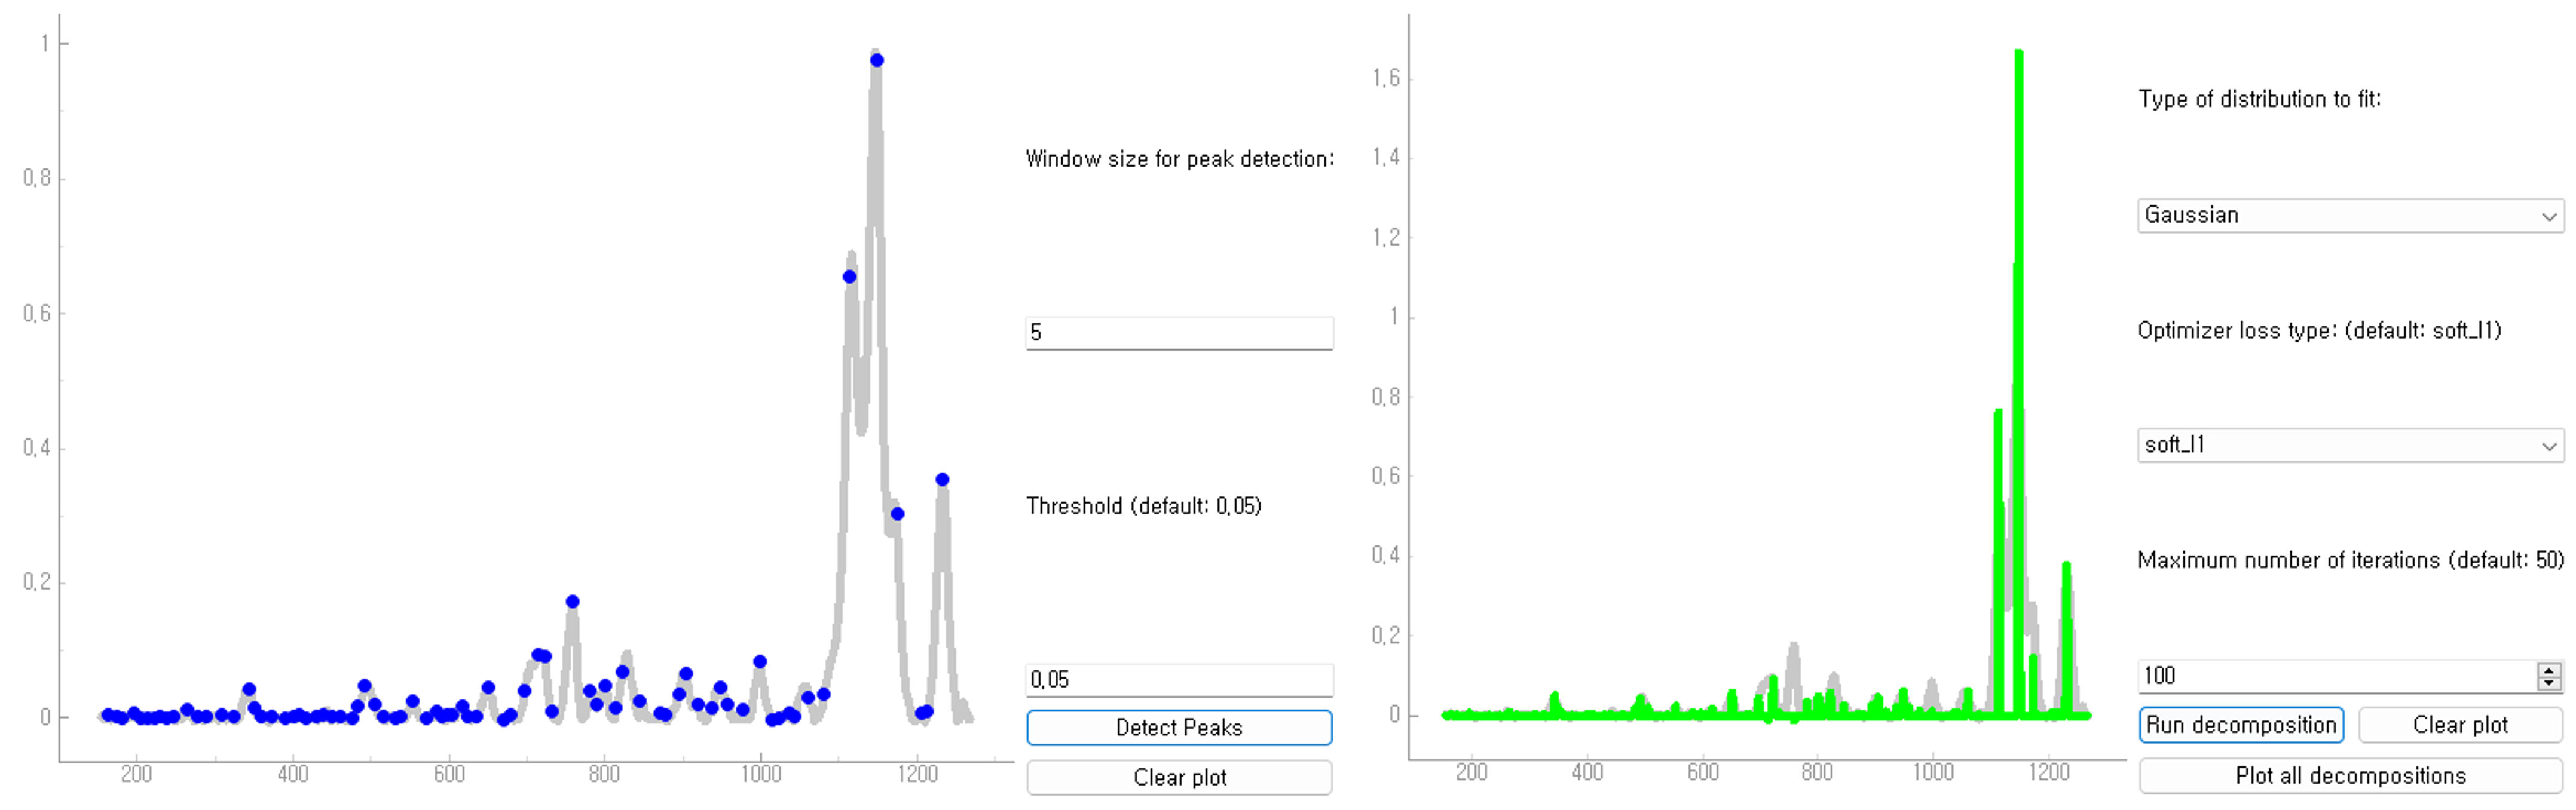
\includegraphics[width=\linewidth]{last_two_windows.png}
    \caption{LEFT: Peak detection window that follows the baseline correction step. The UI is minimalistic with only two parameters to choose: window size and the threshold. RIGHT: Decomposition of the signal into multiple Gaussian distributions. The user can choose one of the three distributions: Gaussian, Lorentzian and Voigt. The optimization loss for the least-squares methods can be chosen from linear, soft l1, Huber loss, and arctan. The green curve shows the Gaussian distributions found by the program.}
    \label{fig:last_two_windows}
\end{figure}

After getting the final decomposition, the following plot in the Figure \ref{fig:abelsonite_final} is obtained.

\begin{figure}
    \centering
    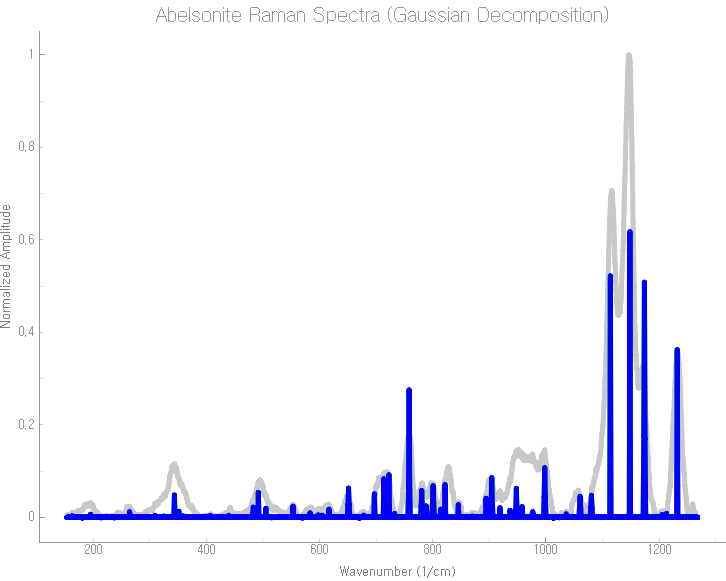
\includegraphics[width=\linewidth]{final_abelsonite.png}
    \caption{The final result obtained by the program shown on the main window of the application.}
    \label{fig:abelsonite_final}
\end{figure}

%
%   
%
\subsection{Usage in the field}
THE APPLICATION WAS USED IN ARIADNI'S WORK, THIS SECTION SHOWS HOW THIS PROGRAM IS TESTED IN THE FIELD USING HER DATA.

%
%   Conclusion
%
\section{Conclusion}

Write some stuff about the outlook:
\begin{itemize}
    \item the backbone of the GUI is presented in this work, but this can be modified further
    \item the program is written in Python 3 to allow as many researchers as possible to collaborate on this work
    \item connecting this program to an embedded system, say with a machine, could reduce the cost of research/experiment significantly.
\end{itemize}

%
%   Acknowledgements
%
\section*{Acknowledgements}

\bibliographystyle{plain}
\bibliography{references} 

\end{document}